\documentclass{article}
\usepackage[utf8]{inputenc}
\usepackage{hyperref,ragged2e,amsmath,multicol,gensymb,setspace,
fancyhdr,amsfonts,tikz,pgfplots,nccmath,enumerate,verbatim}
\usepackage[a4paper, width=216mm, height=297mm, margin=3cm]{geometry}
\usepgfplotslibrary{polar,fillbetween}
\usepgflibrary{shapes.geometric}
\usepgfplotslibrary{external}
\usetikzlibrary{calc,patterns,arrows}
\newcommand\mylog[1]{\mathop{{}^{#1}\mathrm{log}}}
\pgfplotsset{compat=1.15}
\pgfplotsset{my style/.append style={axis x line=middle, axis y line=
middle, xlabel={$x$}, ylabel={$y$}, axis equal }}
\usepackage{etoolbox}
\newcommand{\zerodisplayskips}{%
  \setlength{\abovedisplayskip}{0pt}%
  \setlength{\belowdisplayskip}{0pt}%
  \setlength{\abovedisplayshortskip}{0pt}%
  \setlength{\belowdisplayshortskip}{0pt}}
\pagestyle{fancy}
\fancyhf{}
\lhead{Halaman \thepage}
\rhead{Pembahasan Soal EAS 2020/2021 \\ (\href{https://instagram.com/ahmadzakiyudin_/}{@ahmadzakiyudin\_})}
\hypersetup{
    colorlinks=true,
    linkcolor=blue,
    filecolor=blue,      
    urlcolor=blue,
}
\setlength{\columnsep}{0.8cm}
\begin{document}
 \begin{titlepage}
    \vspace*{\fill}
    \begin{center}
      \Huge {PEMBAHASAN SOAL EAS \\ MATEMATIKA II \\ TAHUN 2020/2021}\\[0.4 cm]
      \huge {Ahmad Hisbu Zakiyudin}
    \end{center}
    \vspace*{\fill}
  \end{titlepage}
\makeatletter
\renewcommand*\env@matrix[1][*\c@MaxMatrixCols c]{%
  \hskip -\arraycolsep
  \let\@ifnextchar\new@ifnextchar
  \array{#1}}
\makeatother
\newcount\arrowcount
\newcommand\arrows[1]{
        \global\arrowcount#1
        \ifnum\arrowcount>0
                \begin{matrix}[c]
                \expandafter\nextarrow
        \fi
}

\newcommand\nextarrow[1]{
        \global\advance\arrowcount-1
        \ifx\relax#1\relax\else \xrightarrow{#1}\fi
        \ifnum\arrowcount=0
                \end{matrix}
        \else
                \\
                \expandafter\nextarrow
        \fi
}
\newpage
\setstretch{1.3}
\section*{SOAL SESI 1 (Kelas 19-44)}
\begin{enumerate}
	\item Dapatkan luas permukaan yang terbentuk, jika kurva $x^2-4x+y^2=0$ yang terletak di kuadran pertama dan diputar pada sumbu$-x$ sepanjang $0\leq x\leq 2$\\
	\textbf{Penyelesaian:}\\
	Tinjau bahwa $x^2-4x+y^2=(x-2)^2+y^2-4=0$ sehingga merupakan persamaan lingkaran yang berpusat di $(2,0)$ dan berjari-jari $2$. Karena terletak pada kuadran pertama dan $0\leq x\leq 2$, maka akan terbentuk seperempat lingkaran dengan jari-jari 2, sehingga jika diputar pada sumbu$-x$ akan terbentuk setengah bola yang luas permukaannya adalah $\dfrac{1}{2}\times 4\pi r^2$. Jadi luas permukaan yang terbentuk adalah $\dfrac{1}{2}\times 4\pi\times 2^2=8\pi$.\\
	Dapat dihitung pula menggunakan integral. Persamaan kurva yang digunakan adalah $y=f(x)=\sqrt{4x-x^2}$ karena $y>0$ pada kuadran pertama. Ingat rumus luas permukaan kurva $y=f(x)$ antara $x=a$ dan $x=b$ terhadap sumbu$-x$ adalah 
	$$ K=\int_a^b 2\pi f(x)\sqrt{1+[f'(x)]^2}\, dx $$
	dengan syarat $f(x)$ kontinu pada $[a,b]$. Tinjau 
	\begin{align*}
	1+[f'(x)]^2 &=1+\left(\dfrac{d}{dx}\sqrt{4x-x^2}\right)^2\\
	&= 1+\left(\dfrac{1}{2\sqrt{4x-x^2}}\times (4-2x)\right)^2\\
	&= 1+\dfrac{x^2-4x+4}{4x-x^2}\\
	&= \dfrac{4}{4x-x^2}
\end{align*}
	Dapat diperoleh luas permukaannya
	\begin{align*}
	K &= \int_0^2 2\pi \sqrt{4x-x^2}\sqrt{\dfrac{4}{4x-x^2}}\, dx\\
	&= \int_0^2 2\pi\times 2\, dx\\
	&= 4\pi x\big|^2_0\\
	&= 8\pi 
\end{align*}		 
	\item Dengan Dalil Guldin I, dapatkan titik berat dataran homogen yang dibatasi kurva $y=\sqrt{1-(x-2)^2}$ dan sumbu$-x$. Sketsa grafiknya.\\
	\textbf{Penyelesaian:}\\
	Tinjau bahwa $y=\sqrt{1-(x-2)^2}$ dapat diubah menjadi $y^2+(x-2)^2=1,~y>0$ merupakan persamaan setengah lingkaran dengan titik pusat lingkarannya adalah $(2,0)$ dan berjari-jari 1. Diperoleh titik berat pada sumbu$-x$ terletak pada $x=2$ sedangkan pada sumbu$-y$ dapat kita cari dengan Dalil Guldin I. Ingat pada Dalil Guldin I berlaku
	$$ V=2\pi \cdot \bar{y}L $$
	dengan $V$ isi benda putar, $\bar{y}$ jarak antara titik berat dataran ke sumbu putar, dan $L$ luas dataran.\\
	Dataran tersebut jika diputar terhadap sumbu$-x$ akan terbentuk sebuah bola dengan volume $\dfrac{4}{3}\pi r^3=\dfrac{4}{3}\pi$. Luas dataran tersebut merupakan luas setengah lingkaran dengan jari-jari 1, yaitu $\dfrac{1}{2}\times \pi r^2=\dfrac{\pi}{2}$. Dapat diperoleh titik berat pada sumbu-$y$ adalah 
	\begin{align*}
	\dfrac{4}{3}\pi &= 2\pi \cdot \bar{y}\cdot \dfrac{\pi}{2}\\
	\bar{y} &= \dfrac{4}{3\pi}
	\end{align*}
	Berikut sketsa grafiknya
	\begin{center}
	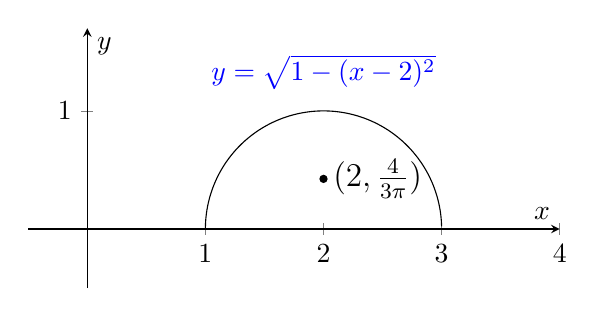
\begin{tikzpicture}
\begin{axis}[
x= 1.5 cm, y=1.5 cm,
 axis lines=middle,
  xmin=-0.5,xmax=4,ymin=-0.5,ymax=1.7,
  xtick distance=1,
  ytick distance=1,
  xlabel=$x$,
  ylabel=$y$]
\addplot [domain=1:3, name path=B,samples=3000] {sqrt(1-(x-2)^2)};
\draw (2,1.1) node[above,blue] {$y=\sqrt{1-(x-2)^2}$};
\fill (2,0.424413) circle(1.5pt) node[right] {\large{$(2,\frac{4}{3\pi})$}};
\end{axis}
\end{tikzpicture}
	\end{center}
	\item \begin{enumerate}
		\item Buatlah sketsa kurva dari persamaan parametrik 
		$$ x=1+\cos t, ~~ y=3-\sin t, ~~ 0\leq t\leq 2\pi $$
		\item Dapatkan panjang busur dari kurva tersebut.
		\item Dapatkan semua nilai parameter $t$ yang menyebabkan kurva tersebut mempunyai garis singgung vertikal 
	\end{enumerate}
	\textbf{Penyelesaian:}
	\begin{enumerate}
		\item Tinjau bahwa $\cos t=x-1$ dan $\sin t=3-y$ sehingga $\cos^2 t+\sin^2 t =1=(x-1)^2+(3-y)^2$ \\Diperoleh persamaan lingkaran yang berpusat di $(1,3)$ dan berjari-jari 1. Karena $0\leq t\leq 2\pi$, maka kurvanya merupakan satu lingkaran penuh sebagai berikut
		\begin{center}
	\begin{tikzpicture}
\begin{axis}[
x= 1 cm, y=1 cm,
 axis lines=middle,
  xmin=-0.5,xmax=3,ymin=-0.5,ymax=4.2,
  xtick distance=1,
  ytick distance=1,
  xlabel=$x$,
  ylabel=$y$]
\draw (1,3) circle[radius=1 cm];
\end{axis}
\end{tikzpicture}
	\end{center}
	\item Karena kurvanya merupakan satu lingkaran penuh dengan jari-jari 1, maka panjang busurnya adalah keliling lingkaran yaitu $2\pi r=2\pi$\\
	Dapat dihitung pula dengan rumus panjang busur untuk kurva parametrik, yaitu 
	$$ S=\int_a^b \sqrt{\left(\dfrac{dx}{dt}\right)^2+\left(\dfrac{dy}{dt}\right)^2}\, dt $$ 
	Tinjau 
	$$ \dfrac{dx}{dt} = -\sin t \text{   dan   } \dfrac{dy}{dt}=-\cos t $$
	serta $a=0$ dan $b=2\pi$ sehingga 
	\begin{align*}
	S &= \int_0^{2\pi}\sqrt{(-\sin t)^2+(-\cos t)^2}\, dt\\
	&= \int_0^{2\pi}\, dt\\
	&= t\big|_0^{2\pi}\\
	&= 2\pi 
	\end{align*}
	\item Kurva tersebut mempunyai garis singgung vertikal jika $\dfrac{dx}{dt}=0$ dan $\dfrac{dy}{dt}\neq 0$, yaitu saat $t=0$, $t=\pi$, dan $t=2\pi$
	\end{enumerate}
	\item Dapatkan panjang busur dari kurva $r=a\cos \theta+b\sin\theta$. (Berikan gambar sketsa kurvanya).\\
	Perhatikan: bilangan $b$ dan $a$ dalam soal ini adalah dua digit terakhir NRP anda. Misalkan NRP anda adalah 06111940000076 maka $b=7$ dan $a=6$, jika $a$ atau $b$ adalah 0 ganti dengan angka 10.\\
	\textbf{Penyelesaian:}\\
	Ingat rumus panjang busur untuk kurva kutub $r=f(\theta)$ jika kurvanya ditelusuri keseluruhan satu kali untuk $\theta$ bergerak dari $\theta=\alpha$ ke $\theta=\beta$ adalah 
	$$ \int_{\alpha}^{\beta}\sqrt{r^2+\left(\dfrac{dr}{d\theta}\right)^2} \, d\theta $$
	Perhatikan bahwa
	\begin{align*}
	r^2 + \left(\dfrac{dr}{d\theta}\right)^2 &= ( a\cos \theta+b\sin\theta)^2+(-a\sin \theta+b\cos\theta)^2\\
	&= a^2\cos^2 \theta+2ab\cos\theta\sin\theta+b^2\sin^2\theta+a^2\sin^2\theta-2ab\sin\theta\cos\theta+b^2\cos^2\theta\\
	&= a^2+b^2
	\end{align*}
	Tinjau bahwa kurva tersebut ditelusuri keseluruhan satu kali untuk $\theta$ bergerak dari $\theta=0$ ke $\theta=\pi$, karena titik $(a,0)$ dan titik $(-a,\pi)$ merupakan titik yang sama dalam koordinat kutub. Jadi diperoleh 
	\begin{align*}
	S &= \int_0^\pi \sqrt{a^2+b^2}\, d\theta\\
	&= \theta\sqrt{a^2+b^2}\big|^\pi_0\\
	&= \pi\sqrt{a^2+b^2} 
	\end{align*}
	Untuk menggambar kurvanya, ingat bahwa $\dfrac{x}{r}=\cos \theta$ dan $\dfrac{y}{r}=\sin \theta$, serta $x^2+y^2=r^2$ sehingga
	\begin{align*}
	r &= a\cos\theta+b\sin\theta\\
	r &= \dfrac{ax}{r}+\dfrac{by}{r}\\
	r^2 &= ax+by\\
	x^2+y^2-ax-by &= 0 \\
	\left(x-\frac{a}{2}\right)^2+\left(y-\frac{b}{2}\right)^2 -\dfrac{a^2}{4}-\dfrac{b^2}{4} &= 0\\
	\left(x-\frac{a}{2}\right)^2+\left(y-\frac{b}{2}\right)^2 &= \dfrac{a^2+b^2}{4}
	\end{align*}
	Jadi kurvanya merupakan lingkaran yang berpusat di $\left(\frac{a}{2},\frac{b}{2}\right)$ dan berjari-jari $\frac{\sqrt{a^2+b^2}}{2}$\\
	Jika $a=6$ dan $b=7$, maka lingkarannya berpusat di $(3,3.5)$ dan berjari-jari $\frac{\sqrt{85}}{2}$, serta memotong titik $(0,0),(6,0),$ dan $(0,7)$ sebagai berikut
	\begin{center}
	\begin{tikzpicture}
\begin{axis}[
x= 0.7 cm, y=0.7 cm,
 axis lines=middle,
  xmin=-1.8,xmax=8,ymin=-1.5,ymax=9,
  xtick={0,3,6},
  ytick={0,3.5,7},
  xlabel=$x$,
  ylabel=$y$]
\draw (3,3.5) circle[radius=0.7*4.60977 cm];
\fill (3,3.5) circle(1.5pt) node[right] {\large{$(3,3.5)$}};
\end{axis}
\end{tikzpicture}
	\end{center}
	Cara lain untuk mendapatkan panjang busurnya adalah menghitung keliling lingkaran tersebut yang berjari-jari $r=\frac{\sqrt{a^2+b^2}}{2}$, yaitu $S=2\pi r=2\pi\frac{\sqrt{a^2+b^2}}{2}=\pi\sqrt{a^2+b^2}$
	\item \begin{enumerate}
		\item Gunakan uji yang sesuai untuk menentukan apakah deret
	$$ \sum_{n=1}^\infty \dfrac{4}{3^n+1} \text{ konvergen atau divergen} $$
		\item Dapatkan jumlahan deret 
		$$ \sum_{k=1}^\infty \left[\dfrac{7}{3^k}+\dfrac{6}{(k+3)(k+4)}\right] $$
	\end{enumerate}
	\textbf{Penyelesaian:}
	\begin{enumerate}
		\item Dengan Prinsip Informal I, suku konstan yaitu 1 pada penyebut dapat dihilangkan tanpa memengaruhi konvergensi deret tersebut, sehingga bentuknya menjadi 
		$$ \sum_{n=1}^\infty \dfrac{4}{3^n} $$
		Bentuk tersebut merupakan deret geometri tak hingga dengan $a=\dfrac{4}{3}$ dan $r=\dfrac{1}{3}$ yang jelas konvergen.
		\item Tinjau bahwa 
		$$ \sum_{k=1}^\infty \left[\dfrac{7}{3^k}+\dfrac{6}{(k+3)(k+4)}\right] = \sum_{k=1}^\infty \dfrac{7}{3^k}+\sum_{k=1}^\infty \dfrac{6}{(k+3)(k+4)}  $$
		Perhatikan bahwa $\displaystyle \sum_{k=1}^\infty \dfrac{7}{3^k} $ merupakan deret geometri tak hingga dengan $a=\dfrac{7}{3}$ dan $r=\dfrac{1}{3}$ sehingga 
		$$ \sum_{k=1}^\infty \dfrac{7}{3^k} = \dfrac{a}{1-r} = \dfrac{\frac{7}{3}}{1-\frac{1}{3}} = \dfrac{7}{2} $$
		Perhatikan pula $\dfrac{6}{(k+3)(k+4)}=6\left(\dfrac{1}{k+3}-\dfrac{1}{k+4}\right)$ sehingga 
		\begin{align*}
		\sum_{k=1}^\infty \dfrac{6}{(k+3)(k+4)} &= \lim_{k\rightarrow \infty} 6\bigg[\left(\dfrac{1}{4}-\dfrac{1}{5}\right)+\left(\dfrac{1}{5}-\dfrac{1}{6}\right)+\left(\dfrac{1}{6}-\dfrac{1}{7}\right)+\cdots \\
		&\qquad \qquad +\left(\dfrac{1}{k+2}-\dfrac{1}{k+3}\right)+\left(\dfrac{1}{k+3}-\dfrac{1}{k+4}\right)\bigg]\\
		&= \lim_{k\rightarrow \infty} 6 \left[\dfrac{1}{4}-\dfrac{1}{k+4}\right]\\
		&= 6\left[\dfrac{1}{4}-0\right]=\dfrac{3}{2}
		\end{align*}
		Jadi 
		$$ \sum_{k=1}^\infty \left[\dfrac{7}{3^k}+\dfrac{6}{(k+3)(k+4)}\right] =\dfrac{7}{2} + \dfrac{3}{2} = 5 $$
	\end{enumerate}
\end{enumerate}
\newpage
\section*{SOAL SESI 2 (Kelas 10-18 dan 45-61)}
\begin{enumerate}
	\item Hitung luas permukaan benda putar dari $y^2-10x+x^2-10y+25=0$ diputar terhadap titik pusat.\\
	\textbf{Penyelesaian:}\\
	Perhatikan bahwa persamaan tersebut dapat diubah menjadi bentuk $(x-5)^2+(y-5)^2=25$ sehingga merupakan lingkaran yang memiliki titik pusat di $(5,5)$ dan berjari-jari $r=5$. Karena benda putarnya diputar terhadap titik pusat, maka akan terbentuk sebuah bola yang luas permukaannya adalah $K=4\pi r^2=4\pi\cdot 5^2=100\pi$
	\item Suatu bidang datar dibatasi oleh kurva $x^2=ay$ dan garis $y=a$
	\begin{enumerate}
		\item Dapatkan pusat massa bidang datar tersebut (Berikan gambar sketsa bidangnya)
		\item Dengan dalil Guldin, hitung volume yang terjadi jika bidang datar pada point (a) tersebut diputar terhadap garis $y=2a$
	\end{enumerate}
	Perhatikan: bilangan $a$ dalam soal ini adalah digit terakhir NRP anda. Misalkan NRP anda adalah 06111940000076 maka $a=6$, jika $a$ adalah 0 ganti dengan angka 10\\
	\textbf{Penyelesaian:}
	\begin{enumerate}
		\item Sketsa dulu bidang datarnya
		\begin{center}
	\begin{tikzpicture}
\begin{axis}[
x= 0.8 cm, y=0.8 cm,
 axis lines=middle,
  xmin=-4,xmax=4,ymin=-0.5,ymax=6,
  xtick={0},
  ytick={0},
  xlabel=$x$,
  ylabel=$y$]
\addplot [domain=-3:3,samples=3000] {x*x/2} node[above] {$x^2=ay$};
\addplot [blue,domain=-3:3,samples=3000] {2} node[below] {$y=a$};
\draw[dashed] (-2,0) -- (-2,2);
\draw (-2,-0.1) node[below] {$-a$};
\draw[dashed] (2,0) -- (2,2);
\draw (2,-0.1) node[below] {$a$};
\end{axis}
\end{tikzpicture}
	\end{center}
	Karena bidang datar tersebut simetris terhadap sumbu$-y$, maka $\bar{x}=0$. \\
	Selanjutnya akan dicari $\bar{y}$. Titik potong kedua kurva pada titik $(-a,a)$ dan $(a,a)$ sehingga batas pengintegralannya dari $x=-a$	sampai $x=a$. Ingat rumus titik berat untuk $\bar{y}$ yaitu
	\begin{align*}
	\bar{y} &= \dfrac{1}{2}\dfrac{\displaystyle \int_a^b (y_1^2-y_2^2)\, dx}{\displaystyle \int_a^b (y_1-y_2)\, dx}
\end{align*}	 
dengan $y_1\geq y_2$ pada $[a,b]$.\\
Dalam soal ini, $y_1=a$ dan $y_2=\dfrac{x^2}{a}$, dapat diperoleh
\begin{align*}
\int_a^b (y_1^2-y_2^2)\, dx &= \int_{-a}^a \left(a^2-\dfrac{x^4}{a^2}\right)\, dx\\
&= a^2x-\dfrac{x^5}{5a^2}\Big|^a_{-a}\\
&= \left(a^3 - \dfrac{a^3}{5}\right)-\left(-a^3+\dfrac{a^3}{5}\right)\\
&= \dfrac{8a^3}{5}\\
\int_a^b (y_1-y_2)\, dx &= \int_{-a}^a \left(a-\frac{x^2}{a}\right)\, dx\\
&= ax-\dfrac{x^3}{3a}\Big|^a_{-a}\\
&= \left(a^2 - \dfrac{a^2}{3}\right)-\left(-a^2+\dfrac{a^2}{3}\right)\\
&= \dfrac{4a^2}{3}
\end{align*}
sehingga
\begin{align*}
\bar{y} &= \dfrac{1}{2}\dfrac{\displaystyle \int_a^b (y_1^2-y_2^2)\, dx}{\displaystyle \int_a^b (y_1-y_2)\, dx}\\
&= \dfrac{1}{2}\dfrac{\frac{8a^3}{5}}{\frac{4a^2}{3}}\\
&= \dfrac{3a}{5}
\end{align*}
Dengan demikian, $Z(\bar{x},\bar{y})=Z(0,\frac{3a}{5})$
	\item Ingat pada Dalil Guldin I berlaku
	$$ V=2\pi \cdot \bar{y}L $$
	dengan $V$ isi benda putar, $\bar{y}$ jarak antara titik berat dataran ke sumbu putar, dan $L$ luas dataran. Karena diputar terhadap garis $y=2a$, maka $\bar{y}$ yang dimaksud adalah $$\bar{y}=2a-\dfrac{3a}{5}=\dfrac{7a}{5}$$. Luas datarannya telah dihitung pada jawaban bagian (a) yaitu $$\displaystyle L=\int_a^b (y_1-y_2)\, dx=\dfrac{4a^2}{3}$$
	Dapat diperoleh
	\begin{align*}
	V=2\pi \cdot \bar{y}L=2\pi \cdot \dfrac{7a}{5}\cdot \dfrac{4a^2}{3} = \dfrac{56a^3\pi}{15}
	\end{align*}
	\end{enumerate}
	\item Buatlah sketsa dan dapatkan panjang kurva yang dibentuk oleh kurva:
	$$ r=\dfrac{2a}{1+\cos \theta}\text{  dan  } r=2a(1+\cos\theta) \text{  di  } 0\leq \theta\leq \frac{\pi}{2} $$
	\textbf{Penyelesaian:}\\
	Transformasikan ke koordinat cartesius untuk membuat sketsa $r_1=\dfrac{2a}{1+\cos\theta}$. Ingat bahwa $\dfrac{x}{r}=\cos\theta$ dan $r^2=x^2+y^2$ sehingga
	\begin{align*}
	r+r\cos\theta &=2a\\
	\sqrt{x^2+y^2}+x &= 2a\\
	x^2+y^2 &= (2a-x)^2\\
	x^2+y^2 &= 4a^2-4ax+x^2\\
	4ax &= 4a^2-y^2\\
	x &= a-\dfrac{y^2}{4a}
	\end{align*}
	yang merupakan kurva parabola mendatar. Untuk $\theta=0$, maka $x=r\cos\theta=r=\dfrac{2a}{1+1}=a$ dan $y=r\sin\theta=0$. Untuk $\theta=\dfrac{\pi}{2}$, maka $x=0$ dan $y=r=\dfrac{2a}{1+0}=2a$. Diperoleh sketsa berikut
	\begin{center}
	\begin{tikzpicture}
\begin{axis}[
x= 1 cm, y=1 cm,
 axis lines=middle,
  xmin=-0.8,xmax=3,ymin=-0.5,ymax=3,
  xtick={0},
  ytick={0},
  xlabel=$x$,
  ylabel=$y$]
\addplot [domain=0:1,samples=3000] {sqrt(4-4*x)};
\draw (1,-0.03) node[below] {$a$};
\draw (-0.03,2) node[left] {$2a$};
\end{axis}
\end{tikzpicture}
	\end{center}
	Sedangkan $r_2=2a(1+\cos\theta)$ merupakan kardioida. Untuk $\theta=0$, maka $x=r\cos\theta=r=2a(1+1)=4a$ dan $y=r\sin\theta=0$. Untuk $\theta=\dfrac{\pi}{2}$, maka $x=0$ dan $y=r=2a(1+0)=2a$. Dapat diperoleh sketsa gabungan kedua kurva sebagai berikut
	\begin{center}
	\begin{tikzpicture}
\begin{axis}[
x= 1 cm, y=1 cm,
 axis lines=middle,
  xmin=-0.8,xmax=5,ymin=-0.5,ymax=3,
  xtick={0},
  ytick={0},
  xlabel=$x$,
  ylabel=$y$]
\addplot [domain=0:1,samples=3000] {sqrt(4-4*x)};
\draw (1,-0.03) node[below] {$a$};
\draw (-0.03,2) node[left] {$2a$};
\addplot[domain=0:90,samples=300,data cs=polar] (x,{2 + 2*cos(x)});
\draw (4,-0.03) node[below] {$4a$};
\end{axis}
\end{tikzpicture}
	\end{center}
	sehingga panjang busur kedua kurva tersebut adalah 
	$$ S_1 = \int_0^{\frac{\pi}{2}} \sqrt{r_1^2+\left(\frac{dr_1}{d\theta}\right)^2}\, d\theta \qquad \text{dan}\qquad S_2 = \int_0^{\frac{\pi}{2}} \sqrt{r_2^2+\left(\frac{dr_2}{d\theta}\right)^2}\, d\theta $$
	Untuk $S_1$, tinjau
	\begin{align*}
	r_1^2+\left(\dfrac{dr_1}{d\theta}\right)^2 &= \left(\dfrac{2a}{1+\cos\theta}\right)^2 + \left(\dfrac{d}{d\theta}\left[\dfrac{2a}{1+\cos\theta}\right]\right)^2\\
	&= \dfrac{4a^2}{(1+\cos\theta)^2} + \left(\dfrac{-2a\sin\theta}{(1+\cos\theta)^2}\right)^2\\
	&= \dfrac{4a^2}{(1+\cos\theta)^2} + \dfrac{4a^2\sin^2\theta}{(1+\cos\theta)^4}\\
	&= \dfrac{4a^2(1+\cos\theta)^2+4a^2\sin^2\theta}{(1+\cos\theta)^4}\\
	&= \dfrac{4a^2+8a^2\cos\theta+4a^2\cos^2\theta+4a^2\sin^2\theta}{(1+\cos\theta)^4}\\
	&= \dfrac{8a^2(1+\cos\theta)}{(1+\cos\theta)^4}\\
	&= \dfrac{8a^2}{(1+\cos\theta)^3}\\
	&= \dfrac{8a^2}{(1+2\cos^2\frac{\theta}{2}-1)^3}\\
	&= \dfrac{a^2}{\cos^6\frac{\theta}{2}} = a^2\sec^6\frac{\theta}{2}
\end{align*}	 
Karena $\sec\frac{\theta}{2}\geq 0$ untuk $0\leq \theta\leq \dfrac{\pi}{2}$, maka 
$$ S_1 = \int_0^\frac{\pi}{2} \sqrt{a^2\sec^6\frac{\theta}{2}}\, d\theta =\int_0^\frac{\pi}{2} a\sec^3\frac{\theta}{2}\, d\theta$$
Selanjutnya akan dihitung integral tak tentu 
$$ I = \int \sec^3 u \, du $$
dengan mengggunakan rumus reduksi
$$ \int \sec^n x\, dx = \dfrac{\sec^{n-2}x\tan x}{n-1}+\dfrac{n-2}{n-1}\int \sec^{n-2} x\, dx $$ 
sehingga
\begin{align*}
 I = \int\sec^3 u\, du &= \dfrac{\sec u\tan u}{2}+\dfrac{1}{2}\int \sec u\, du
\end{align*}
Selanjutnya hitung
\begin{align*}
I_1 &= \int\sec u\, du\\
&= \int \dfrac{\sec u(\sec u+\tan u)}{\sec u+\tan u}\, du\\
&= \int\dfrac{\sec^2 u+\sec u\tan u}{\sec u+\tan u}\, du
\end{align*}
Misalkan $p=\sec u+\tan u$ sehingga $dp = (\sec^2 u +\sec u\tan u) \, du$ sehingga
\begin{align*}
I_1 &= \int \dfrac{1}{p}\, dp\\
&= \ln |p| + C_1\\
&= \ln |\sec u +\tan u| + C_1
\end{align*}
Jadi 
$$ I = \dfrac{\sec u\tan u+\ln |\sec u+\tan u|}{2}+C $$
Misalkan $\dfrac{\theta}{2}=u$ sehingga $d\theta=2\, du$ dan batas atasnya menjadi $u=\dfrac{\pi}{4}$ sedangkan batas bawahnya tetap $u=0$, diperoleh
\begin{align*}
S_1 = \int_0^\frac{\pi}{2} a\sec^3\frac{\theta}{2}\, d\theta &= 2a\int_0^\frac{\pi}{4}\sec^3 u \, du\\
&= 2a\left[\dfrac{\sec u\tan u+\ln |\sec u+\tan u|}{2}\right]^\frac{\pi}{4}_0\\
&= 2a\left[\dfrac{(\sqrt{2})(1)+\ln|\sqrt{2}+1|}{2}-\dfrac{(1)(0)+\ln|1+0|}{2}\right]\\
&= a(\sqrt{2}+\ln|1+\sqrt{2}|)
\end{align*}
Selanjutnya untuk $S_2$, tinjau
\begin{align*}
r_2^2+\left(\dfrac{dr_2}{d\theta}\right)^2 &= (2a(1+\cos\theta))^2+\left(\dfrac{d}{d\theta}[2a(1+\cos\theta)]\right)^2\\
&= 4a^2(1+2\cos\theta +\cos^2\theta)+\left(2a(-\sin\theta)\right)^2\\
&= 4a^2+8a^2\cos\theta +4a^2\cos^2\theta+4a^2\sin^2\theta\\
&= 8a^2(1+\cos\theta)\\
&= 8a^2(1+2\cos^2\frac{\theta}{2}-1)\\
&= 16a^2\cos^2\frac{\theta}{2}
\end{align*}
Karena $\cos\frac{\theta}{2}\geq 0$ untuk $0\leq \theta\leq \dfrac{\pi}{2}$, maka
\begin{align*}
S_2 &= \int_0^\frac{\pi}{2}\sqrt{16a^2\cos^2\frac{\theta}{2}}\, d\theta\\
&= \int_0^\frac{\pi}{2}4a\cos\frac{\theta}{2}\, d\theta\\
&= (4a)(2)\sin\frac{\theta}{2}\Big|^\frac{\pi}{2}_0\\
&= 8a\cdot\dfrac{1}{2}\sqrt{2}-0 = 4a\sqrt{2}
\end{align*}
Jadi panjang keseluruhan kurva yang dimaksud adalah \begin{align*}
S=S_1+S_2 &= a\sqrt{2}+a\ln|1+\sqrt{2}|+4a\sqrt{2}\\
&= a(5\sqrt{2} +\ln|1+\sqrt{2}|)
\end{align*}
	\item Selesaikan 
	\begin{enumerate}
		\item Tentukan konvergensi barisan $\left\{ n\sin\frac{\pi}{n}\right\}^\infty_{n=1}$;\\
		Dari jawaban tersebut, tentukan konvergensi $\left\{ \dfrac{n^2}{2n+1}\sin\dfrac{\pi}{n}\right\}^\infty_{n=1}$
		\item Dengan uji perbandingan, tentukan deret berikut konvergen ataukah divergen?
		$$ \sum_{n=0}^\infty \dfrac{2^n\sin^2(5n)}{4^n+\cos^2 n} $$
	\end{enumerate}
	\textbf{Penyelesaian:}
	\begin{enumerate}
		\item Akan dicari $\displaystyle \lim_{n\rightarrow +\infty} n\sin \frac{\pi}{n}=L_1$\\ Misalkan $\dfrac{1}{n}=k$, maka $k\rightarrow 0^+$ karena $n\rightarrow +\infty$, sehingga
		$$ L_1=\lim_{k\rightarrow 0^+} \dfrac{\sin \pi k}{k} = \pi $$ 
		Jadi barisan $\left\{ n\sin\frac{\pi}{n}\right\}^\infty_{n=1}$ konvergen ke $\pi$\\
		Selanjutnya tinjau, 
		$$ \dfrac{n^2}{2n+1}\sin \frac{\pi}{n}=\dfrac{n}{2n+1}\times n\sin\frac{\pi}{n}$$ 
		Dapat diperoleh $\displaystyle \lim_{n\rightarrow +\infty} \dfrac{n}{2n+1}=\lim_{n\rightarrow +\infty} \dfrac{1}{2+\frac{1}{n}}=\dfrac{1}{2}= L_2$\\
		Akibatnya $$ \lim_{n\rightarrow +\infty} \dfrac{n^2}{2n+1}\sin \frac{\pi}{n} = \lim_{n\rightarrow +\infty} \dfrac{n}{2n+1}\cdot \lim_{n\rightarrow +\infty} n\sin \frac{\pi}{n} = L_1\cdot L_2=\dfrac{\pi}{2} $$
		Jadi barisan $\left\{ \dfrac{n^2}{2n+1}\sin\dfrac{\pi}{n}\right\}^\infty_{n=1}$ konvergen ke $\dfrac{\pi}{2}$
		\item Tinjau bahwa $0\leq \sin^2(5n)\leq 1$ sehingga $2^n\sin^2(5n)\leq 2^n$\\
		Tinjau pula $0\leq \cos^2 n\leq 1$ sehingga $4^n\leq 4^n+\cos^2 n$ dan $\dfrac{1}{4^n+\cos^2 n}\leq \dfrac{1}{4^n}$\\
		Akibatnya 
		$$ \dfrac{2^n\sin^2(5n)}{4^n+\cos^2 n} \leq \dfrac{2^n}{4^n} = \dfrac{1}{2^n} $$
		Karena $\displaystyle \sum_{n=0}^\infty \dfrac{1}{2^n}$ merupakan deret geometri tak hingga dengan $a=1$ dan $r=\dfrac{1}{2}$ yang jelas konvergen sehingga deret $\displaystyle \sum_{n=0}^\infty \dfrac{2^n\sin^2(5n)}{4^n+\cos^2 n}$ juga konvergen.
	\end{enumerate}
	\item Buktikan $\displaystyle \sum_{k=2}^\infty \dfrac{1}{k(\ln k)^p}$ konvergen jika $p>1$\\
	\textbf{Penyelesaian:}\\
	Uji konvergensi deret tersebut dengan uji integral berikut
	\begin{align*}
	\int_2^\infty \dfrac{1}{x(\ln x)^p}\, dx
	\end{align*}
	Misalkan $\ln x=u$ sehingga $\dfrac{1}{x}\, dx=du$, akan dihitung dulu integralnya tanpa menggunakan batas integral
	\begin{align*}
	\int \dfrac{1}{x(\ln x)^p}\, dx &= \int \dfrac{1}{u^p} \,du\\
	&= \int u^{-p} \, du\\
	&= \dfrac{u^{1-p}}{1-p}\\
	&= \dfrac{(\ln x)^{1-p}}{1-p}
	\end{align*}
	Dapat diperoleh 
	\begin{align*}
	\int_2^\infty \dfrac{1}{x(\ln x)^p}\, dx &= \lim_{a\rightarrow\infty} \int_2^a \dfrac{1}{x(\ln x)^p}\, dx\\
	&= \lim_{a\rightarrow\infty} \left(\dfrac{(\ln a)^{1-p}}{1-p}-\dfrac{(\ln 2)^{1-p}}{1-p}\right)\\
	&= \dfrac{1}{1-p}\left( \lim_{a\rightarrow\infty} \dfrac{1}{(\ln a)^{p-1}}-\dfrac{1}{(\ln 2)^{p-1}}\right)
	\end{align*}
	Jika $p>1$, diperoleh
	 $$\dfrac{1}{1-p}\left( \lim_{a\rightarrow\infty} \dfrac{1}{(\ln a)^{p-1}}-\dfrac{1}{(\ln 2)^{p-1}}\right) = \dfrac{1}{1-p}\left(0-\dfrac{1}{(\ln 2)^{p-1}}\right) = \dfrac{1}{(p-1)(\ln 2)^{p-1}}$$
	Dapat disimpulkan deret tersebut konvergen jika $p>1$\\
	Jika $p<1$, maka $p-1<0$ sehingga
	 $$\dfrac{1}{1-p}\left( \lim_{a\rightarrow\infty} \dfrac{1}{(\ln a)^{p-1}}-\dfrac{1}{(\ln 2)^{p-1}}\right) = \infty$$
	Dapat disimpulkan deret tersebut divergen jika $p<1$
\end{enumerate}
\newpage
\section*{SOAL SESI 3 (Kelas 1-9 dan 62-70)}
\begin{enumerate}
	\item Dapatkan panjang kurva $y=75\cosh \frac{x}{75}$ dari $x=-150$ ke $x=150$\\
	\textbf{Penyelesaian:}\\
	Ingat bahwa panjang kurva $y=f(x)$ dari $x=a$ ke $x=b$ dan $f(x)$ kontinu pada $[a,b]$ adalah 
	$$ S=\int_a^b \sqrt{1+[f'(x)]^2}\, dx $$
	Tinjau 
	\begin{align*}
	1+[f'(x)]^2 &= 1+\left(\dfrac{d}{dx}\left[75\cosh \left(\frac{x}{75}\right)\right]\right)^2\\
	&= 1+\left(75\sinh^2 \left(\frac{x}{75}\right)\cdot \dfrac{1}{75}\right)^2\\
	&= 1+\sinh^2 \left(\frac{x}{75}\right)\\
	&= \cosh^2\left(\frac{x}{75}\right)
	\end{align*}
	Karena $y=75\cosh \frac{x}{75}$ kontinu pada $[-150,150]$ dan nilainya selalu positif, maka 
	\begin{align*}
	S &= \int_{-150}^{150} \sqrt{\cosh^2\left(\frac{x}{75}\right)} \, dx\\
	&= \int_{-150}^{150} \cosh \left(\frac{x}{75}\right) \, dx\\
	&= 75\sinh\left(\frac{x}{75}\right)\Big|^{150}_{-150}\\
	&= 75(\sinh(2)-\sinh(-2))\\
	&= 75(\sinh(2)+\sinh(2))\\
	&= 150\sinh(2)
	\end{align*}
	\item Diberikan persamaan kurva $x=2\sqrt{1-y};~-1\leq y\leq 0$
	\begin{enumerate}
		\item Buatlah sketsa grafik persamaan kurvanya
		\item Dapatkan luas permukaan benda putar jika kurva diputar terhadap sumbu $y$
	\end{enumerate}
	\textbf{Penyelesaian:}
	\begin{enumerate}
		\item Perhatikan bahwa persamaan tersebut dapat diubah menjadi bentuk $x^2=4-4y$ atau $y=\dfrac{4-x^2}{4}$ yang merupakan persamaan parabola dengan $-1\leq y\leq 0$ dan $x\geq 0$. Untuk $y=-1$ diperoleh $x=2\sqrt{2}$ dan untuk $y=0$ diperoleh $x=2$ sebagai berikut
		\begin{center}
	\begin{tikzpicture}
\begin{axis}[
x= 1.2 cm, y=1.2 cm,
 axis lines=middle,
  xmin=0,xmax=3.5,ymin=-1.5,ymax=1,
  xtick ={0,2},
  ytick distance=1,
  xlabel=$x$,
  ylabel=$y$]
\addplot [domain=2:2.82842712),samples=3000] {(4-x*x)/4)};
\end{axis}
\end{tikzpicture}
	\end{center}
	\item Untuk luas permukaan benda putar yang terbentuk, dapat digunakan persamaan yang diberikan pada soal yaitu $x=g(y)=2\sqrt{1-y}$ dengan $-1\leq y\leq 0$. Ingat rumus luas permukaan benda putar dari kurva yang diputar terhadap sumbu$-y$ yaitu
	$$ K= \int_a^b 2\pi g(y)\sqrt{1+[g'(y)]^2}\, dy $$
	Dapat diperoleh 
	\begin{align*}
	K &= \int_{-1}^0 2\pi (2\sqrt{1-y})\sqrt{1+\left(\dfrac{d}{dx}\left[2\sqrt{1-y}\right]\right)^2} \, dy\\
	&= 4\pi \int_{-1}^0 \sqrt{1-y}\sqrt{1+\left(\dfrac{-1}{\sqrt{1-y}}\right)^2}\, dy\\
	&= 4\pi \int_{-1}^0 \sqrt{1-y}\sqrt{\dfrac{1-y+1}{1-y}}\, dy\\
	&= 4\pi \int_{-1}^0 \sqrt{2-y}\, dy\\
	&= 4\pi \left[-\dfrac{2}{3}(2-y)^{3/2}\right]^0_{-1}\\
	&= -\dfrac{8\pi}{3}\left[2\sqrt{2}-3\sqrt{3}\right]\\
	&= \dfrac{8\pi}{3}\left[3\sqrt{3}-2\sqrt{2}\right]
	\end{align*}
	\end{enumerate}
	\item Diberikan partikel bergerak sepanjang kurva $\begin{cases}x=1-t\\ y=\sqrt{8+2t-t^2}\end{cases}$ dengan $-2\leq t\leq 1$
	\begin{enumerate}
		\item Nyatakan dalam persamaan kutub $r=f(\theta)$ dengan lintasan $\theta$
		\item Tentukan panjang lintasan kurva tersebut
		\item Sketsa persamaan kurva tersebut dan arah lintasannya 
	\end{enumerate}
	\textbf{Penyelesaian:}
	\begin{enumerate}
		\item Perhatikan bahwa $t=1-x$ sehingga
		\begin{align*}
		y&=\sqrt{8+2(1-x)-(1-x)^2}\\
		&=\sqrt{8+2-2x-1+2x-x^2}\\
		&= \sqrt{9-x^2}
		\end{align*}
		Ingat bahwa $y=r\sin\theta$ dan $x=r\cos\theta$ sehingga
		\begin{align*}
		r\sin\theta &=\sqrt{9-r^2\cos^2\theta}\\
		r^2\sin^2\theta &= 9-r^2\cos^2\theta\\
		r^2 &= 9
		\end{align*}
		Dapat diambil $r=f(\theta)=3$. Untuk $t=-2$, maka $x=r\cos\theta=3$ sehingga $\theta=0$, dan untuk $t=1$, maka $x=r\cos\theta=0$ sehingga $\theta=\dfrac{\pi}{2}$. Jadi $r=f(\theta)=3$ dengan $0\leq \theta\leq\dfrac{\pi}{2}$
		\item Tinjau bahwa $r=3$ dengan $0\leq \theta\leq \dfrac{\pi}{2}$ merupakan seperempat lingkaran dengan jari-jari $r=3$ di kuadran pertama, sehingga panjang lintasan kurva tersebut merupakan seperempat keliling lingkaran yaitu $\dfrac{1}{4}\cdot 2\pi r=\dfrac{3}{2}\pi$
		\item Dari jawaban (b) sudah diperoleh bentuk kurvanya.\\
		Sedangkan untuk arah lintasannya, tinjau bahwa $x$ berkurang dan $y$ bertambah ketika $t$ bergerak dari $-2$ ke 1, sehingga arahnya berlawanan arah jarum jam. Berikut sketsanya
		\begin{center}
	\begin{tikzpicture}
\begin{axis}[
x= 1.4 cm, y=1.4 cm,
 axis lines=middle,
  xmin=-0.5,xmax=3.5,ymin=-0.5,ymax=3.5,
  xtick distance=1,
  ytick distance=1,
  xlabel=$x$,
  ylabel=$y$]
\addplot[domain=0:90,samples=300,data cs=polar] (x,{3});
\end{axis}
\end{tikzpicture}
	\end{center}
	\end{enumerate}
	\item Selesaikan:
	\begin{enumerate}
		\item Diberikan $\{a_n\}^\infty_{n=1}$ dengan $a_n=\dfrac{1}{n^2}+\dfrac{3}{n^2}+\dfrac{5}{n^2}+\cdots +\dfrac{2n-1}{n^2}$\\
		Tuliskan 5 suku pertama barisan, dan dapatkan $\displaystyle \lim_{n\rightarrow \infty} a_n$
		\item Jika diberikan barisan $(a_n)=(0,1,0,1,0,1,\dots)$ dan $(b_n)=(1,0,1,0,1,0,\dots)$ maka selidiki tentang konvergensi dari: $1. (a_n+b_n);\quad 2. (a_n\cdot b_n);\quad 3. \left(\dfrac{a_n}{b_n}\right)$
	\end{enumerate}
	\textbf{Penyelesaian:}
	\begin{enumerate}
		\item Tinjau bahwa 
		$$ a_n = \dfrac{1+3+5+\cdots +(2n-1)}{n^2} =\dfrac{\frac{n}{2}(1+(2n-1))}{n^2}=1$$
		untuk $n=1,2,3,\cdots$. Diperoleh $(a_n)=(1,1,1,\dots)$ sehingga $a_1=a_2=a_3=a_4=a_5=1$ merupakan 5 suku pertama barisan tersebut dan $\displaystyle \lim_{n\rightarrow \infty} a_n=1$ 
		\item \begin{enumerate}
		\item Tinjau $(a_n+b_n)=(1,1,1,\dots)$ sehingga barisan tersebut konvergen ke 1
		\item Tinjau $(a_n\cdot b_n)=(0,0,0,\dots)$ sehingga barisan tersebut konvergen ke 0
		\item Tinjau untuk $n=2$, $\dfrac{a_n}{b_n}$ tidak terdefinisi sehingga konvergensi barisan $\left(\dfrac{a_n}{b_n}\right)$ tidak dapat ditentukan
		\end{enumerate}
	\end{enumerate}
	\item Diketahui fungsi $f(x)=\dfrac{1}{1-ax}$
	\begin{enumerate}
		\item Dapatkan deret Maclaurin dari $f(x)$ (Nyatakan dalam notasi sigma)
		\item Gunakan hasil dari (a) untuk mendapatkan deret Maclaurin dari fungsi $f(x)=\dfrac{1}{(1-ax)^2}$
	\end{enumerate}
	Perhatikan: bilangan $a$ dalam soal ini adalah digit terakhir NRP anda. Misalkan NRP anda adalah 06111940000076 maka $a=6$, jika $a=0$ ganti dengan angka 10.\\
	\textbf{Penyelesaian:}
	\begin{enumerate}
		\item Tinjau 
		\begin{multicols}{2}
		\begin{align*}
		f(x) &= \dfrac{1}{1-ax}\\
		f'(x) &= \dfrac{a}{(1-ax)^2}\\
		f''(x) &= \dfrac{a\cdot 2a}{(1-ax)^3}\\
		f'''(x) &= \dfrac{a\cdot 2a\cdot 3a}{(1-ax)^4}\\
		&~~\vdots\\
		f^{(k)}(x) &= \dfrac{a\cdot 2a\cdot 3a\cdots ka}{(1-ax)^{k+1}} = \dfrac{k!a^k}{(1-ax)^{k+1}}
		\end{align*}
		\begin{align*}
		f(0) &= 1\\
		f'(0) &= a\\
		f''(0) &= a\cdot 2a\\
		f'''(0) &= a\cdot 2a\cdot 3a\\
		&~~\vdots\\
		f^{(k)}(0) &= a\cdot 2a\cdot 3a\cdots ka=k!a^k
		\end{align*}
		\end{multicols}
		Diperoleh deret Maclaurin dari $f(x)$
		\begin{align*}
		\sum_{k=0}^\infty \dfrac{f^{(k)}(0)}{k!}x^k &= f(0) + f'(0)x +\dfrac{f''(0)}{2!}x^2+\cdots+\dfrac{f^{(k)}(0)}{k!}x^k+\cdots\\
		&= 1+(a)(x)+\dfrac{2!a^2}{2!}x^2+\cdots+\dfrac{k!a^k}{k!}x^k+\cdots\\
		&= 1+(ax)+(ax)^2+\cdots (ax)^k+\cdots\\
		&= \sum_{k=0}^\infty (ax)^k
\end{align*}				 
		Alternatif penyelesaian dengan metode substitusi.\\
		Tinjau deret Maclaurin dari $\displaystyle \dfrac{1}{1-x}=1+x+x^2+x^3+\cdots=\sum_{k=0}^\infty x^k$. Dengan metode substitusi diperoleh deret Maclaurin dari $f(x)$ adalah 
		$$ \dfrac{1}{1-ax}=1+ax+(ax)^2+(ax)^3+\cdots =\sum_{k=0}^\infty (ax)^k$$
		\item Tinjau $\dfrac{d}{dx}(ax)^k=ka(ax)^{k-1}$ sehingga
	\begin{align*}
	\dfrac{d}{dx} \left(\dfrac{1}{1-ax}\right) &= \dfrac{d}{dx} \sum_{k=0}^\infty (ax)^k\\
	\dfrac{a}{(1-ax)^2} &= \sum_{k=0}^\infty ka(ax)^{k-1}\\
	\dfrac{a}{(1-ax)^2} &= a\sum_{k=0}^\infty k(ax)^{k-1}\\
	\dfrac{1}{(1-ax)^2} &= \sum_{k=0}^\infty k(ax)^{k-1} = 1+2(ax)+3(ax)^2+\cdots 
	\end{align*}
	\end{enumerate}
\end{enumerate}
\end{document}
